% ------------------------------------------------------------------------
% file `c3-exercise-2-exercise-body.tex'
%   in folder `xsim/'
%
%     exercise of type `exercise' with id `2'
%
% generated by the `exercise' environment of the
%   `xsim' package v0.21 (2022/02/12)
% from source `c3' on 2022/06/12 on line 42
% ------------------------------------------------------------------------
    L'entraîneur de l'équipe de football de Sésaville compare le nombre de tirs effectués par ses
    trois attaquants pendant la première moitié du championnat.
    \begin{center}
        \pgfplotsset{width=.35\linewidth}
        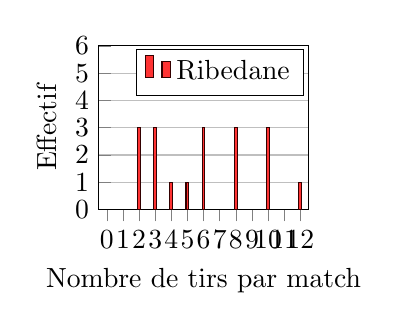
\begin{tikzpicture}
    \begin{axis}[
            ybar,
            xmin=-0.5,
            ymin=0,
            xmax=12.5,
            ymax=6,
            xlabel=Nombre de tirs par match,
            ylabel=Effectif,
            bar width=1pt,
            %major grid style={draw=black},
            ymajorgrids = true,
            xtick pos=bottom,
            ytick pos=left,
            %minor y tick num = 4,
            %minor y tick style = {transparent},
            %major x tick style = {transparent},
            %yminorticks = true,
            %yminorgrids = true,
            xtick distance=1,
            ytick distance=1,
            %axis lines* = left
        ]
        \addplot[red!20!black,fill=red!80!white] coordinates{
                (2,3)
                (3,3)
                (4,1)
                (5,1)
                (6,3)
                (8,3)
                (10,3)
                (12,1)
            };
        \legend{Ribedane}
    \end{axis}
\end{tikzpicture}
        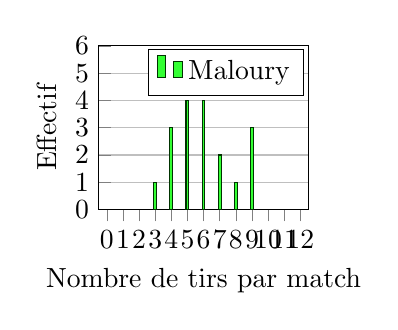
\begin{tikzpicture}
    \begin{axis}[
        ybar,
        xmin=-0.5,
        ymin=0,
        xmax=12.5,
        ymax=6,
        xlabel=Nombre de tirs par match,
        ylabel=Effectif,
        bar width=1pt,
        %major grid style={draw=black},
        ymajorgrids = true,
        xtick pos=bottom,
        ytick pos=left,
        %minor y tick num = 4,
        %minor y tick style = {transparent},
        %major x tick style = {transparent},
        %yminorticks = true,
        %yminorgrids = true,
        xtick distance=1,
        ytick distance=1,
        %axis lines* = left
    ]
        \addplot[green!20!black,fill=green!80!white] coordinates{
               (3,1)
               (4,3)
               (5,4)
               (6,4)
               (7,2)
               (8,1)
               (9,3)
            };
            \legend{Maloury}
    \end{axis}
\end{tikzpicture}
        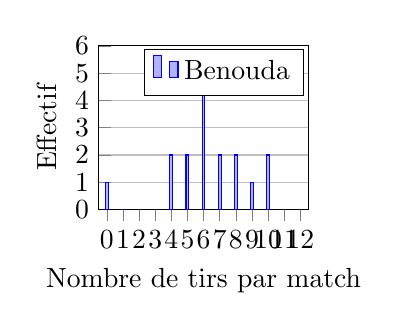
\begin{tikzpicture}
    \begin{axis}[
        ybar,
        xmin=-0.5,
        ymin=0,
        xmax=12.5,
        ymax=6,
        xlabel=Nombre de tirs par match,
        ylabel=Effectif,
        bar width=1pt,
        %major grid style={draw=black},
        ymajorgrids = true,
        xtick pos=bottom,
        ytick pos=left,
        %minor y tick num = 4,
        %minor y tick style = {transparent},
        %major x tick style = {transparent},
        %yminorticks = true,
        %yminorgrids = true,
        xtick distance=1,
        ytick distance=1,
        %axis lines* = left
    ]
        \addplot coordinates{
                (0,1)
                (1,0)
                (4,2)
                (5,2)
                (6,5)
                (7,2)
                (8,2)
                (9,1)
                (10,2)
            };
            \legend{Benouda}
    \end{axis}
\end{tikzpicture}
    \end{center}
    %\pgfplotsset{width=.5\linewidth}

    \begin{enumerate}
        \item Calcule le nombre de tirs au but moyen par match des trois attaquants.
        \item Interprète ce résultat par rapport au contexte.
        \item  Détermine le nombre de tirs médian pour chacune de ces trois séries.
        \item Interprète ce résultat par rapport au contexte.
    \end{enumerate}
